\documentclass{article}
\usepackage{amsmath}
\providecommand{\brak}[1]{\ensuremath{\left(#1\right)}}
\usepackage{graphicx}
\usepackage{circuitikz}
\graphicspath{{./figs}}
\begin{document}
\textbf{Q.46} In the circuit shown below, a positive edge-triggered D flip-flop is used for sampling input data $ D_{in} $ using clock CK.The XOR gate outputs 3.3 volts for logic HIGH and 0 volts for logic LOW levels.The data bit and clock periods are equal and the value of $ \Delta T / T_{ck} $ = 0.15,where the parameters $ \Delta T $ and $ T_ck$ are shown in the figure.Assume that the Flip and the XOR gate are ideal.
\begin{figure}[!ht]
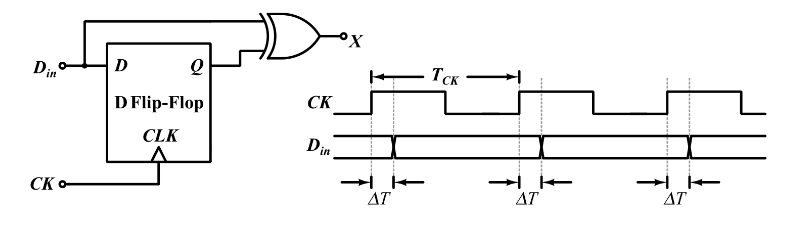
\includegraphics[scale=0.4]{figs/image.png}
\end{figure}
\end{document}
